\documentclass[12pt]{article}

\usepackage[margin=1in]{geometry}
\usepackage{xcolor}
\usepackage{graphicx}
\usepackage{url}
\usepackage{hyperref}

\newcommand\TODO[1]{\textcolor{red}{#1}}
\newcommand\todo[1]{\textcolor{red}{#1}}

\begin{document}
\title{Fine-grained Access for Securing NFC:  Distributed Key Association}
\author{Max Feldman \and Stephanie Rogers \and Richard Xia}
\maketitle

\section{Abstract}
Near Field Communication (NFC) is a form of contactless communication which allows devices to transfer data over radio; it is similar to RFID, but with a much smaller range of use.
NFC has existed for some time, but its implementation in Android phones, along with an API for developers, has only recently gained popularity.
Upon scanning an NFC tag, Android will automatically run the application which has been associated with the type of data on that tag, sometimes without user interaction or approval.
The Android NFC API offers application developers a new, more powerful means to access NFC capabilities in mobile devices, but this introduces an increased attack space and additional potential for vulnerability.
Android provides access to an NFC Data Exchange Format (NDEF) API, but does not offer any of the various security measures which have been proposed.

We examine the growing space of NFC applications offered for Android, and provide a cursory categorization of the functionality and general security practices of these applications.
Alarmingly, several applications implement features such as SMS messaging or calling given phone numbers, or accessing arbitrary URLs, which are provided by an NFC tag without even prompting the user.
We attempt to address the issue of resource access on behalf of external data, in the context of NFC.
We discuss known issues and vulnerabilities with NDEF security, and how our proposal mitigates some of these concerns.
We also keep in mind the importance of usability, especially in applications which must perform quickly and smoothly--as is the case with NFC applications. Finally, we present the description of a user study which can effectively evaluate the tradeoffs between secure access control and usability.

\TODO{\section{Introduction}}
1-2 page version of paper

\section{Background}
\todo{mention NDEF TNF, type (maybe show a bit level NDEF record layout)}
Near Field Communication (NFC) is an emerging technology for wireless communication which allows NFC-enabled devices to transfer small amounts of data at a close proximity, usually no more than a few centimeters.
At the most basic level, NFC specifies a set of protocols for this wireless communication based off of the radio-frequency identification (RFID) standards.
NFC offers current and predicted functionality of contactless transactions, data exchange and an alternative to traditional contactless technologies such as RFID and QR codes.
Aimed at mobile phones, devices use NFC in two ways, labeled active and passive mode.
In passive mode, there is a device actively generating a radio frequency (RF) field that initiates contact to the passive NFC tag.
In this case, the device can read or write information stored on NFC tags and cards without the passive targets needing any power source.
Additionally, NFC phones have the ability to communicate with other NFC-enabled mobile phones to transfer data peer-to-peer in active mode.
In this case both devices are generating their own RF fields.

\subsection{Android NFC}

The Android system sends and receives NFC data in the form of NFC Data Exchange Format (NDEF) messages. These messages, which are stored in the NFC tag, act as a container for one or more NDEF records which are further broken up into a header and a payload, which contain typed data such as MIME-type media, a URI or a custom application payload.

\begin{figure}[h!]
\begin{minipage}{\textwidth}
	\centering
		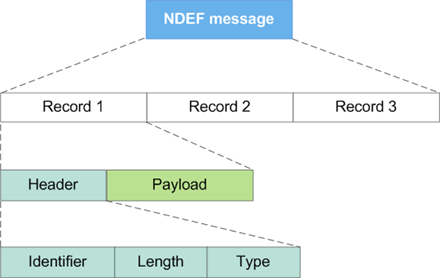
\includegraphics[width=0.5\textwidth]{NDEF_Format.png}
	\caption[Caption for LOF]%
		{NDEF Message Format\footnote{\url{http://www.developer.nokia.com/Community/Wiki/Understanding_NFC_Data_Exchange_Format_(NDEF)_messages}}}

\end{minipage} 
\end{figure}

Specifically, the Android system offers the ability to read and write NFC tags for passive mode, and beam NDEF messages from one device to another with Android Beam\footnote{\url{http://developer.android.com/guide/topics/connectivity/nfc/nfc.html}} for active mode. 

\subsection{Android Intents}
The core components of an Android application are activated through messages called intents.\footnote{\url{http://developer.android.com/guide/components/intents-filters.html}}
Intents are used for inter-application and intra-application communication by sending messages with relevant information about operations to be performed to various applications.  

When NFC is enabled and the screen is unlocked, Android devices will always be searching for input from an NFC tag or device. 
When the device discovers an NFC tag, the Android OS creates an intent which is dispatched to an application which has registered for it.
This information is processed by Android's special tag dispatch system to determine which activity to launch.
In the case that more than one application can handle the type of data contained in the tag, the phone will open a prompt for the user to choose among the several applications; however, if there is only one application, the phone will automatically launch this application and process the tag.
NFC input can force Android phones (with certain settings) to parse images, videos, contacts, and office documents, call or text arbitrary phone numbers, establish bluetooth connections, and open web pages via the browser, all without user interaction.  

\subsection{Android Permission System}
Android applications run in a sandbox which allows areas of the system to be isolated and thus limit access to the security-related parts of the Android API.
However, access to these resources can be granted to an application if the developer requests the appropriate permissions in the application's manifest.
Android developers are expected to use least-privilege with their permission requests: limit the permissions requested to only those that are absolutely necessary for the function of their applications. 
\TODO{Relate this back to NFC.}

\section{Threat Model}
While NFC is still an emerging technology, there are several vulnerabilities which can afflict applications.
In our work, we address three of these: malicious NFC tags, more generally, fraudulent data inputs, and threats on user privacy.
\subsection{Malicious Tags}
We define a malicious NFC tag as an NFC tag which contains data that would cause a user to act on data which they did not expect.
If the attacker has the ability to automatically have the phone call a specified number, then a tolled number could easily be inserted and thus result in a monetary loss on the part of the user. 
This is a direct and obvious vulnerability in any application the calls an arbitrary phone number specified by a tag.
An example of an application that does so is Samsung's Tectile application which, when scanning a tag with a phone number and directions to call this number, will do so without any further consideration. \TODO{Is this true? Have we actually tried doing this? And we should put a link to the app page here}
For example, an attacker could replace the tag on a poster advertising a local event with a new tag, containing a paid phone number.
When a user swipes the tag to view the event's website, their phone will place a call and their account will be billed.
\subsection{Fraudulent data inputs}
\TODO{How is this different than malicious tags?}
Fraudulent data inputs refer to tags and other means of inputting NFC data which is not intended.
For example, this applies to an attacker initiating an NFC connection handover, which results in malicious data transfer from the attacker's phone to the victim's.

\TODO{This is for 294, and should possibly be omitted from other versions}
\subsection{Privacy Concerns}
Several NFC applications have the possibility of writing information to an NFC tag.
This means that users have the ability to write anything they want to their own tags.
It may be beneficial for some users to use these tag writing applications to write sensitive or critical information to tags they keep in specific locations.
However, if encryption is not used, an attacker who can gain access to these tags will have unfettered access to their information.
NFC is also used as a means of initiating connections on higher-bandwidth media (eg. bluetooth), but if this connection handover is interfered with then an attacker may be able to listen in on the new connection.

There are several other threats to consider, which we mention here, but are outside the scope of our project.

\subsection{Eavesdropping}
In ``Securing Near Field Communication'' \cite{kortvedt2009}, Kortvedt, proves that it is possible to eavesdrop on NFC communication using simple equipment and methods.
Since the NFC communication protocol does not offer any security or encryption itself, it is up to the developer to implement or use encryption to secure the data within the application's code. 
\subsection{Relay, Replay, Denial of Service}
A relay attack results when the attacker positions himself between a sender and receiver of information.
However, the sender and receiver may not be aware that they are actually communicating with each other.
\TODO{describe this? are these descriptions worth it}
A replay attack consists of an attacker listening to data transmitted by a victim, and using that information again at a later time.
Denial of service in the case of NFC applications would result in preventing NFC transactions from occurring.
This could come from exploiting logic flaws in NFC applications, or merely jamming radio transmissions, for example.
We omit discussion of these attacks from our paper.

\todo{himself or herself}
Relay, replay, and denial of service attacks are omitted from our discussion as well.

\TODO{\subsection{Current Solutions}}
Related NFC Technology and Security - authenticating tags rather than users

* MiFare: hardware that allows the locking of data and allows symmetric mutual authentication of users and write protection to defend against reading and writing of the tag (privacy)

* FeliCa: authentication and write protection 

* AFAICT: lock the data (not overwritable), but no authentication!

* Signature NDEF Records

* Certificates 

\subsubsection{ \TODO{Dump of things from related work}}
\textbf{Application level attacks.}
Kerschberger\cite{kerschberger2011} presents an overview of NFC security and vulnerabilities.


\textbf{Network-level attacks.}

One major foray into the analysis of network-level NFC vulnerabilities was presented by Charlie Miller at BlackHat 2012\cite{miller2012}.
Miller employs fuzz testing to show that carefully crafted NFC payloads can do much more than just crash a device---in some cases phones can be forced to parse arbitrary data or open web pages without user interaction.
Miller's work provides a wide analysis of the NFC attack surface, but our research will seek to provide much more depth in the exploration of application-level vulnerabilities.

RFID, a precursor to and superset of NFC, has also raised several security issues in the past.
Though RFID is a much older technology, it is remains relevant as both the foundation for NFC, and as a technology which is still employed in various applications (most prominently touch-activated credit cards).
Heydt-Benjamin et al.\cite{heydtbenjamin2007} discuss issues involved in early generation deployments of RFID credit cards, and were successfully able to initiate various attacks on three major RFID enabled credit cards (including attacks which access private information or enable arbitrary purchases by the attacker).
Such attacks remain important considerations due to the growing prominence of smartphone payment applications  (such as Google Wallet), so we keep all of these vulnerabilities in mind as we explore NFC security vulnerabilities.
This paper presents some countermeasures, but some may be impractical (such as shielding) and others can be improved upon due to more flexible computing options of smartphones.

Haselsteiner et al\cite{haselsteiner2006} discuss general security issues with NFC (beyond the scope of just mobile phones).
The paper discusses threats of eavesdropping, data corruption, data modification, data insertion, and man-in-the-middle attacks (though MITM is dismissed as practically impossible).
The paper recommends establishing a secure channel between devices in order to prevent such attacks, and provides valuable discussion of how this channel would work.
The paper does not, however, provide an implementation (as the purpose of the paper was to illustrate general NFC issues).
As our focus is restricted to Android devices, we have the ability to recommend and implement Android-specific solutions.

Francis et al.\cite{francis2012} discuss the potential for relay attacks on NFC transactions, and implement a software version of this attack which can be used on an NFC-enabled device.
A relay attack exploits the assumption that two devices engaged in an NFC transaction are actually adjacent (by placing a proxy in between the two devices).
This is a serious potential exploit which must be defended against by any security-conscious application (as it may allow for arbitrary credit card purchases, for example).
The paper suggests several potential counters to such attacks; our analysis examines how popular applications employ relay-attack countermeasures, and to what degree they are effective.

\textbf{Random shit}
Analysis of smartphone applications in general (though we restrict our focus to Android devices, as iPhones do not yet offer NFC) is a much more thoroughly explored field, and several projects provide valuable insight into application testing.

%While RFID technology and Android application analysis have both been explored, there has been very limited exploration of Android-specific NFC applications, and their potential vulnerabilities.
%We leverage this previous exploration to provide large-scale analysis of NFC applications, vulnerabilities, and coding practices, as well as to recommend best practices for preventing NFC attacks.

\TODO{anything in analysis goes into background}
%\section{Analysis of Apps}
%* Intro: Why analyze
%** general coding practices re: NFC
%** what practices contribute to vulnerabilities of NFC apps
%** As for as we know, no broad analysis of NFC app level stuff
%** provide suggestion for NFC app devs (we are in a unique position in that this tech is up and coming)

%\subsection{Application Characteristics}
%*** tiny - have a specific function and only does one specific thing given a tag. These only require a small subset of permissions. 
%\\
%*** superapps - use a lot of permissions and perform several different actions ranging from reading and writing tags, to handling monetary transactions, performing actions on the phone, or transferring musics, pictures, or other data.
%
%\subsection{Static Analysis}
%* static
%\subsubsection{Permissions}
%* current apps, what permissions do they use - ML Classifier here
%\subsubsection{Taint Tracking}
%trace where data read from NFC tags is ended
%** other static tools? 
%\subsubsection{Crypto/Eavesdropping}
%\TODO{Eavesdropping - Talk about more in analysis portion when we discuss the use of crypto within application's code - the fact that developers aren't using known crypto libraries means they are either implementing crypto themselves or not securing their data at all} 
%** Overwriting tags- do apps in general 0 out prior data, or not?
%
%\subsection{Dynamic Analysis - might not exist}
%* dynamic
%** taintdroid
%** droidblaze
%
%\subsection{Manual Analysis}
%* manual
%** looked at source code of ~10 applications
%** played with apps
%** trace exec paths if possible
%** BEAM
%*** If you scan an app, it'll take you to the app store

\section{Related Work}
%Close range radio wave communication has existed for some time, but the application of NFC in mobile phones is a recent development and still growing in popularity.
The NFC Forum\footnote{\url{http://www.nfc-forum.org/}}, which publishes NFC standards\footnote{\url{http://www.nfc-forum.org/specs/spec_list/}} and best practices, was only formed in 2004.
The relative youth of this field has resulted in many aspects remaining largely unexplored.
In this section we present relevant past work in the area of NFC security, as well as mobile phone application security in general.

\textbf{Pre-shared keys.}
One approach for authenticating tags is to share keys between tag readers and tag writers.
Kortvedt \cite{kortvedt2009} proposes a general framework for providing one-way and mutual authentication over NFC, but requires the use of pre-shared keys.
He suggests using a centralized key authority associated with mobile carriers such as Over-The-Air (OTA) programming or SMS for distributing keys.
We believe is impractical and inappropriate for all types of applications given that tag authors may be distinct from application authors and may wish to distribute keys.
There is also no notion of trust, as a user must trust that the key being shared is legitimate.
We instead seek to provide a decentralized mechanism for trusting and granting trust to a user-defined set of NFC tag authors.

\textbf{Signatures and Certificates.}
The NFC Signature Record Type Definition (RTD), which can be used to sign NDEF records, was standardized to deal with threats caused by malicious tags including spoofing, phishing and denial of service.
Using signatures on a tag causes a performance and space penalty, which are important since NFC tag readers are mobile devices and NFC tags themselves have very limited storage space \cite{kilas2009}.
The standard now focuses on being able to authenticate the source of data through a certificate authority which distributes and validates public keys \cite{rosati2011}.
However, several vulnerabilities arise with these signature regarding the \textit{authorization} of tags and the authentication of unsigned and the combination of unsigned tags and tags signed by different authors \cite{roland2010,roland2011}.
We propose a way for users to authorize keys based on the data type and application, which are enough to determine a fixed behavior (e.g. calling a phone number from a tag, opening a URL stored on a tag).


\section{Proposed Solution}
\todo{make ``tag author'' more general}
We propose a system of controlling the access that NFC inputs are granted by the Android OS.
This access control system aims to provide a simple and usable means for phone users to grant access to certain capabilities to trusted tag authors.
A capability in this case refers to the ability to access a system resource, such as to call a phone or open a URL.
We differentiate this from a permission (which individual applications must request), in that it is more restrictive, and specific to a tag author (as identified by their public key).
This system uses per-application access control to specify approved, unapproved, and unencountered access-requestors.
We specify the goals and non-goals of our system and then outline the approach in detail, as well as discuss our implementation.
\subsection{Goals}
The principal goal of this system is to allow users to link their trust with their access policies.
The user's trust should define the access granted to external entities.
If a user trusts a particular tag author to provide non-malicious URLs, then the user can grant that tag author approval for all URLs in the context of that application.
This system must be fast and unobtrusive, so that the short duration of an NFC interaction is not impeded.
The system must also be simple, for both users and application developers.
Users should be able to understand what access policies they choose to grant, and administer these policies with ease.
This includes granting additional access and revoking existing access.
\subsection{Non-goals}
We do not seek to provide trust mechanisms for users.
At best, we wish to leverage existing trust mechanisms (such as certificates included in Signed NDEF records), but present the information regarding the identity of an author in an easy-to-read format.
If the signer of a tag is identified in a certificate chain, then it is important to present the user with that identity so that the user can make an informed decision regarding access control.
We do not seek to offer integrity or authentication.
These are both goals of the NDEF Signature RTD, and as such we leverage these properties but do not duplicate the effort of providing them.
This system does not offer an alternative to the certificate scheme support by the NDEF Signature RTD.
\subsection{Approach}
In order to provide fine-grained access control, each application maintains its own access control list.
An entry in this list consists of the TNF of the NDEF record, the Type of the NDEF record, and the public key extracted from the signature which applies to that record.
This system is intended to be an OS library which allows developers to grant, revoke, and verify access within the context of their application.
When a tag is read, its data will be marshalled to the appropriate application, if that application is not already running.
\subsubsection{Verifying Access}
Before an application acts on NDEF input data, it verifies that the NDEF record's type and public key (from the associated signature record) exist in the access control list.
The OS provides a method call which allows the application developer to easily check whether this content author has been approved.
This content author can either be approved for a specific type (TNF and Type field), or for all types.
For example, an author with public key Ka may have a record /[001:55:Ka/], indicating that their key is trusted for all URI inputs within the context of that application.
Another author with public key Kb may have a record /[*:*:Kb/], indicating that they will always be granted access by this application.
If the lookup of \todo{how to phrase this?} /[TNF:TYPE:Key/] returns true, then the data's provider has been granted access and operation proceeds uninterrupted.
If the lookup fails, then a user will be prompted to either allow the operation to proceed once (ie. without granting permanent access), grant permanent access, or deny access and abort the operation.
\subsubsection{Granting Access}
If a user elects to grant access upon receipt of NDEF data, then they will be given the option of granting the input author permanent access for that NDEF type (TNF and Type fields), or for all types (a wildcard match on the TNF and Type fields).
The OS will then attempt to deliver the most readable identifier of the public key which the user is about to approve.
In most cases, extracting the identifying information from the certificate will be sufficient to present the user with a concise identity of the content author.
The user then chooses the type of access they wish to grant to that public key, and this access choice is written to the access control list for that app.
\subsubsection{Revoking Access}
\todo{make this better}
Users will be provided an interface to the access control lists for their applications by the OS.
Through this interface, the user can view all authors to which they have granted access (including the human-readable name associated with the public key).
The user can then choose to revoke access to an author by removing associated entries of that author in relevant lists.
The user can also remove only one access grant to an author, if they so choose.
Revocation should additionally support certificate revocation lists; ie. if a tag with a revoked certificate is encountered, that revocation should propagate to the access control list.
Additionally, if a certificate has been found which is outside its validity period, the access associated with that identity should be revoked.


\subsection{Alternatives}
One access control method we considered was requiring approval when data was handed over to another process, as opposed to approval upon 

\section{Implementation}
We implemented our access control system as an Android library that Android developers can include and access in their projects.
Our current implementation provides both means of writing and reading tags using our authentication scheme, allowing developers of both tag-reading and tag-writing applications to benefit from increased security.
We present this implementation as a proof-of-concept; ideally, such additions to the Android NFC stack would be implemented at OS-level.
There are several advantages to kernel modifications, which are discussed below.


\subsection{Key Management}
Users need to be able to add and remove keys from their base of trusted authors (either manually, or through a tag reader application).
For our API, we use Android's \texttt{SharedPreferences}, which provides persistent key-value storage.
Our current implementation provides a unique instance of this key storage (a \texttt{KeyFile}) to an individual application (ie. a given application can only access and modify its own keys).
Key sharing between applications is a useful feature which would be simpler to implement securely at OS-level.
When a user reads a tag, the tag's signature record will either contain a public key in its entirety, or contain a URI pointer to a public key.
If this public key has been added to the Key File, it is considered trusted, otherwise, the user must add this key.
\TODO{``tag providers''? or ``tag authors''? what should we name them?}
When a user writes a tag using this API, the private key for the phone is accessed and a ECDSA signature is generated and appended.

\subsection{Application Flow}
On instantiation, a \texttt{SignedNdef} object will attempt to open up the list of authorized keys saved on the Android device.
We do not seek to provide trust mechanisms for users.
At best, we wish to leverage existing trust mechanisms (such as certificates included in Signed NDEF records), 
It provides methods for opening, closing, reading, and writing NDEF-formatted tags by delegating to a private instance of the \texttt{Ndef} class.
In addition, it will automatically enforce the security protocols described earlier.
When reading a tag, it will query the \texttt{KeyManager} to find a public key which matches the signature of the signed Ndef tag.
If it can locate a valid public key which matches the signature, it will transparently return the non-signature records on the tag.
In case of any errors, failure to verify the signature or failure to locate a valid public key, reading the tag will throw an exception.
\TODO{include figure for application flow}

\subsection{Cryptographic protocols}
\todo{this is an issue with SignedNDEF}
One issue regarding the storage of additional authentication data on an NFC tag is the limited size of the tag.
NDEF Signatures support various signature algorithms, with ECDSA among them.
ECDSA is able to use smaller keys to provide the same security as DSA with a larger key.
For example, a 160-bit ECDSA key provides the same security level as a 1024-bit DSA key.
\TODO{verify the above, which is from wikipedia}

\subsection{Recommendations for Kernel Implementation}
Implementing this scheme at OS-level will allow for simpler sharing of keys between applications, by providing a single, shared Key File.
We recommend an additional application permission in order to make a modification of this Key File; this will provide greater control over which applications have been granted permission to influence the set of trusted tag authors.
This implementation would also allow Android itself to display messages to the user, in order to centralize and standardize any necessary error reporting or warnings.

\TODO{\section{Evaluation}}
\subsection{Space Performance}
It has an overhead of this many bytes... 
\subsection{Usability}
\subsection{Security}
* simplicity/overhead for user (warning message?)
* how many apps can benefit from this?
* applicability
** do 3 case studies (examples of applying it to an application)
** do it on github
* How many additional lines of code required for using API?

* (performance (time+space))
* security of this scheme
** bits of security (e.g. signature size)
** assumptions/foundations (e.g. secure key distribution)
** key storage on Android phones can't be tampered with

* LIMITATIONS

* key add/revoke
** app perm to add
** app perm to remove
** done via syscalls, i.e. android holds this
*** some intent?
** some way for app developer to add centralized repo of keys
** automatic get key

* Does phone already have a pub key pair?
* backwards compatibility
** Read NDEF standards and how Android handles them

brainstorm                         works for                           bad
- NDEF record/type for signature   updated os
                                   app viewing finite \# records
- length exclused signature        above                               violates standards
  + above                          app viewing variable \# of records   

%Possible things to consider when measuring security
%- Economy of mechanism. Designs which are smaller and simpler are easier to inspect and trust.
%- Fail-safe defaults. By default, access should be denied unless it is explicitly granted.
%- Complete mediation. Every access to every object should be checked.
%- Least privilege. Every program should operate with the minimum set of privileges necessary to do its job. This prevents accidental mistakes becoming security problems.
%- Least common mechanism. Anything which is shared among different programs can be a path for communication and a potential security hole, so as little data as possible should be shared.
%- Accountability. The system should be able to accurately record “who” is responsible for using a particular privilege.
%- Psychological acceptability. The system should not place an undue burden on its users. Several other practical issues arise when designing a security system for Java.
%- Performance. We must consider how our designs constrain system performance. Security checks which must be performed at run-time will have performance costs.
%- Compatibility. We must consider the number and depth of changes necessary to integrate the security system with the existing Java virtual machine and standard libraries. Some changes may be impractical.
%- Remote calls. If the security system can be extended cleanly to remote method invocation, that would be a benefit for building secure, distributed systems.



\TODO{\section{Future Work}}
* compression/optimization
* OS perms, kernel mods to support this
* application sharing and how to do this well

\subsection{Recommended User Study}
There are several potential use cases for the NFC technology which have yet to be established. It is important to consider the usability of a solution such as ours for the various cases in which the technology could be used. Thus, we suggest a user study to test the obstrusiveness and effectiveness of access controls in a realistic setting. 

Using human participants, the study would attempt to measure the overhead imposed by warnings/approvals presented by our proposed system as well as the effectiveness in blocking against the given attacks, taking into consideration the ability for the user to fall for the attack. There are several implementation choices on the part of the developer which would be of interest to observe. We suggest trying two main implementation approaches, including pop up menus to ask the user for their approval for each given tag, as well as incorporating untrusted tags as a warning into the phone rather than blatant pop ups. Things like how often the warning were ignored and in what cases they were ignored should be measured during the experiment in order to provide insight into the effectiveness of the system. Asking the users a series of questions after their tests, including which tags they believed to be malicious and how easy or intuitive the access control scheme presented was to use would offer additional insight to the usability. 

\subsection{Optimization}

\subsection{Application Sharing}

\TODO{\section{Conclusion}}

\TODO{\section{Acknowledgements}}

\TODO{\section{References}}

\bibliographystyle{abbrv}
\bibliography{cs261}

\end{document}
